% TEMPLATE for Usenix papers, specifically to meet requirements of
%  USENIX '05
% originally a template for producing IEEE-format articles using LaTeX.
%   written by Matthew Ward, CS Department, Worcester Polytechnic Institute.
% adapted by David Beazley for his excellent SWIG paper in Proceedings,
%   Tcl 96
% turned into a smartass generic template by De Clarke, with thanks to
%   both the above pioneers
% use at your own risk.  Complaints to /dev/null.
% make it two column with no page numbering, default is 10 point

% Munged by Fred Douglis <douglis@research.att.com> 10/97 to separate
% the .sty file from the LaTeX source template, so that people can
% more easily include the .sty file into an existing document.  Also
% changed to more closely follow the style guidelines as represented
% by the Word sample file. 

% Note that since 2010, USENIX does not require endnotes. If you want
% foot of page notes, don't include the endnotes package in the 
% usepackage command, below.

% This version uses the latex2e styles, not the very ancient 2.09 stuff.
\documentclass[letterpaper,twocolumn,10pt]{article}
\usepackage{usenix,epsfig,endnotes}
\usepackage{graphicx,calc,subfigure,caption,float}
\usepackage[breaklinks,colorlinks]{hyperref}
\usepackage{endnotes,microtype,xspace,fancyvrb,multirow}
\usepackage{array,underscore,relsize}
\usepackage{booktabs,amsmath}

\renewcommand{\ttdefault}{pxtt}

\newcommand{\URL}{\url}
\newcommand{\cc}[1]{\mbox{\smaller[0.5]\texttt{#1}}}

%\clubpenalty=10000
%\widowpenalty=10000

%\linespread{1.2}

\fvset{fontsize=\scriptsize,xleftmargin=8pt,numbers=left,numbersep=5pt}


\makeatletter
\def\PY@reset{\let\PY@it=\relax \let\PY@bf=\relax%
    \let\PY@ul=\relax \let\PY@tc=\relax%
    \let\PY@bc=\relax \let\PY@ff=\relax}
\def\PY@tok#1{\csname PY@tok@#1\endcsname}
\def\PY@toks#1+{\ifx\relax#1\empty\else%
    \PY@tok{#1}\expandafter\PY@toks\fi}
\def\PY@do#1{\PY@bc{\PY@tc{\PY@ul{%
    \PY@it{\PY@bf{\PY@ff{#1}}}}}}}
\def\PY#1#2{\PY@reset\PY@toks#1+\relax+\PY@do{#2}}

\expandafter\def\csname PY@tok@gd\endcsname{\def\PY@tc##1{\textcolor[rgb]{0.63,0.00,0.00}{##1}}}
\expandafter\def\csname PY@tok@gu\endcsname{\let\PY@bf=\textbf\def\PY@tc##1{\textcolor[rgb]{0.50,0.00,0.50}{##1}}}
\expandafter\def\csname PY@tok@gt\endcsname{\def\PY@tc##1{\textcolor[rgb]{0.00,0.27,0.87}{##1}}}
\expandafter\def\csname PY@tok@gs\endcsname{\let\PY@bf=\textbf}
\expandafter\def\csname PY@tok@gr\endcsname{\def\PY@tc##1{\textcolor[rgb]{1.00,0.00,0.00}{##1}}}
\expandafter\def\csname PY@tok@cm\endcsname{\let\PY@it=\textit\def\PY@tc##1{\textcolor[rgb]{0.25,0.50,0.50}{##1}}}
\expandafter\def\csname PY@tok@vg\endcsname{\def\PY@tc##1{\textcolor[rgb]{0.10,0.09,0.49}{##1}}}
\expandafter\def\csname PY@tok@m\endcsname{\def\PY@tc##1{\textcolor[rgb]{0.40,0.40,0.40}{##1}}}
\expandafter\def\csname PY@tok@mh\endcsname{\def\PY@tc##1{\textcolor[rgb]{0.40,0.40,0.40}{##1}}}
\expandafter\def\csname PY@tok@go\endcsname{\def\PY@tc##1{\textcolor[rgb]{0.53,0.53,0.53}{##1}}}
\expandafter\def\csname PY@tok@ge\endcsname{\let\PY@it=\textit}
\expandafter\def\csname PY@tok@vc\endcsname{\def\PY@tc##1{\textcolor[rgb]{0.10,0.09,0.49}{##1}}}
\expandafter\def\csname PY@tok@il\endcsname{\def\PY@tc##1{\textcolor[rgb]{0.40,0.40,0.40}{##1}}}
\expandafter\def\csname PY@tok@cs\endcsname{\let\PY@it=\textit\def\PY@tc##1{\textcolor[rgb]{0.25,0.50,0.50}{##1}}}
\expandafter\def\csname PY@tok@cp\endcsname{\def\PY@tc##1{\textcolor[rgb]{0.74,0.48,0.00}{##1}}}
\expandafter\def\csname PY@tok@gi\endcsname{\def\PY@tc##1{\textcolor[rgb]{0.00,0.63,0.00}{##1}}}
\expandafter\def\csname PY@tok@gh\endcsname{\let\PY@bf=\textbf\def\PY@tc##1{\textcolor[rgb]{0.00,0.00,0.50}{##1}}}
\expandafter\def\csname PY@tok@ni\endcsname{\let\PY@bf=\textbf\def\PY@tc##1{\textcolor[rgb]{0.60,0.60,0.60}{##1}}}
\expandafter\def\csname PY@tok@nl\endcsname{\def\PY@tc##1{\textcolor[rgb]{0.63,0.63,0.00}{##1}}}
\expandafter\def\csname PY@tok@nn\endcsname{\let\PY@bf=\textbf\def\PY@tc##1{\textcolor[rgb]{0.00,0.00,1.00}{##1}}}
\expandafter\def\csname PY@tok@no\endcsname{\def\PY@tc##1{\textcolor[rgb]{0.53,0.00,0.00}{##1}}}
\expandafter\def\csname PY@tok@na\endcsname{\def\PY@tc##1{\textcolor[rgb]{0.49,0.56,0.16}{##1}}}
\expandafter\def\csname PY@tok@nb\endcsname{\def\PY@tc##1{\textcolor[rgb]{0.00,0.50,0.00}{##1}}}
\expandafter\def\csname PY@tok@nc\endcsname{\let\PY@bf=\textbf\def\PY@tc##1{\textcolor[rgb]{0.00,0.00,1.00}{##1}}}
\expandafter\def\csname PY@tok@nd\endcsname{\def\PY@tc##1{\textcolor[rgb]{0.67,0.13,1.00}{##1}}}
\expandafter\def\csname PY@tok@ne\endcsname{\let\PY@bf=\textbf\def\PY@tc##1{\textcolor[rgb]{0.82,0.25,0.23}{##1}}}
\expandafter\def\csname PY@tok@nf\endcsname{\def\PY@tc##1{\textcolor[rgb]{0.00,0.00,1.00}{##1}}}
\expandafter\def\csname PY@tok@si\endcsname{\let\PY@bf=\textbf\def\PY@tc##1{\textcolor[rgb]{0.73,0.40,0.53}{##1}}}
\expandafter\def\csname PY@tok@s2\endcsname{\def\PY@tc##1{\textcolor[rgb]{0.73,0.13,0.13}{##1}}}
\expandafter\def\csname PY@tok@vi\endcsname{\def\PY@tc##1{\textcolor[rgb]{0.10,0.09,0.49}{##1}}}
\expandafter\def\csname PY@tok@nt\endcsname{\let\PY@bf=\textbf\def\PY@tc##1{\textcolor[rgb]{0.00,0.50,0.00}{##1}}}
\expandafter\def\csname PY@tok@nv\endcsname{\def\PY@tc##1{\textcolor[rgb]{0.10,0.09,0.49}{##1}}}
\expandafter\def\csname PY@tok@s1\endcsname{\def\PY@tc##1{\textcolor[rgb]{0.73,0.13,0.13}{##1}}}
\expandafter\def\csname PY@tok@sh\endcsname{\def\PY@tc##1{\textcolor[rgb]{0.73,0.13,0.13}{##1}}}
\expandafter\def\csname PY@tok@sc\endcsname{\def\PY@tc##1{\textcolor[rgb]{0.73,0.13,0.13}{##1}}}
\expandafter\def\csname PY@tok@sx\endcsname{\def\PY@tc##1{\textcolor[rgb]{0.00,0.50,0.00}{##1}}}
\expandafter\def\csname PY@tok@bp\endcsname{\def\PY@tc##1{\textcolor[rgb]{0.00,0.50,0.00}{##1}}}
\expandafter\def\csname PY@tok@c1\endcsname{\let\PY@it=\textit\def\PY@tc##1{\textcolor[rgb]{0.25,0.50,0.50}{##1}}}
\expandafter\def\csname PY@tok@kc\endcsname{\let\PY@bf=\textbf\def\PY@tc##1{\textcolor[rgb]{0.00,0.50,0.00}{##1}}}
\expandafter\def\csname PY@tok@c\endcsname{\let\PY@it=\textit\def\PY@tc##1{\textcolor[rgb]{0.25,0.50,0.50}{##1}}}
\expandafter\def\csname PY@tok@mf\endcsname{\def\PY@tc##1{\textcolor[rgb]{0.40,0.40,0.40}{##1}}}
\expandafter\def\csname PY@tok@err\endcsname{\def\PY@bc##1{\setlength{\fboxsep}{0pt}\fcolorbox[rgb]{1.00,0.00,0.00}{1,1,1}{\strut ##1}}}
\expandafter\def\csname PY@tok@kd\endcsname{\let\PY@bf=\textbf\def\PY@tc##1{\textcolor[rgb]{0.00,0.50,0.00}{##1}}}
\expandafter\def\csname PY@tok@ss\endcsname{\def\PY@tc##1{\textcolor[rgb]{0.10,0.09,0.49}{##1}}}
\expandafter\def\csname PY@tok@sr\endcsname{\def\PY@tc##1{\textcolor[rgb]{0.73,0.40,0.53}{##1}}}
\expandafter\def\csname PY@tok@mo\endcsname{\def\PY@tc##1{\textcolor[rgb]{0.40,0.40,0.40}{##1}}}
\expandafter\def\csname PY@tok@kn\endcsname{\let\PY@bf=\textbf\def\PY@tc##1{\textcolor[rgb]{0.00,0.50,0.00}{##1}}}
\expandafter\def\csname PY@tok@mi\endcsname{\def\PY@tc##1{\textcolor[rgb]{0.40,0.40,0.40}{##1}}}
\expandafter\def\csname PY@tok@gp\endcsname{\let\PY@bf=\textbf\def\PY@tc##1{\textcolor[rgb]{0.00,0.00,0.50}{##1}}}
\expandafter\def\csname PY@tok@o\endcsname{\def\PY@tc##1{\textcolor[rgb]{0.40,0.40,0.40}{##1}}}
\expandafter\def\csname PY@tok@kr\endcsname{\let\PY@bf=\textbf\def\PY@tc##1{\textcolor[rgb]{0.00,0.50,0.00}{##1}}}
\expandafter\def\csname PY@tok@s\endcsname{\def\PY@tc##1{\textcolor[rgb]{0.73,0.13,0.13}{##1}}}
\expandafter\def\csname PY@tok@kp\endcsname{\def\PY@tc##1{\textcolor[rgb]{0.00,0.50,0.00}{##1}}}
\expandafter\def\csname PY@tok@w\endcsname{\def\PY@tc##1{\textcolor[rgb]{0.73,0.73,0.73}{##1}}}
\expandafter\def\csname PY@tok@kt\endcsname{\def\PY@tc##1{\textcolor[rgb]{0.69,0.00,0.25}{##1}}}
\expandafter\def\csname PY@tok@ow\endcsname{\let\PY@bf=\textbf\def\PY@tc##1{\textcolor[rgb]{0.67,0.13,1.00}{##1}}}
\expandafter\def\csname PY@tok@sb\endcsname{\def\PY@tc##1{\textcolor[rgb]{0.73,0.13,0.13}{##1}}}
\expandafter\def\csname PY@tok@k\endcsname{\let\PY@bf=\textbf\def\PY@tc##1{\textcolor[rgb]{0.00,0.50,0.00}{##1}}}
\expandafter\def\csname PY@tok@se\endcsname{\let\PY@bf=\textbf\def\PY@tc##1{\textcolor[rgb]{0.73,0.40,0.13}{##1}}}
\expandafter\def\csname PY@tok@sd\endcsname{\let\PY@it=\textit\def\PY@tc##1{\textcolor[rgb]{0.73,0.13,0.13}{##1}}}

\def\PYZbs{\char`\\}
\def\PYZus{\char`\_}
\def\PYZob{\char`\{}
\def\PYZcb{\char`\}}
\def\PYZca{\char`\^}
\def\PYZam{\char`\&}
\def\PYZlt{\char`\<}
\def\PYZgt{\char`\>}
\def\PYZsh{\char`\#}
\def\PYZpc{\char`\%}
\def\PYZdl{\char`\$}
\def\PYZhy{\char`\-}
\def\PYZsq{\char`\'}
\def\PYZdq{\char`\"}
\def\PYZti{\char`\~}
% for compatibility with earlier versions
\def\PYZat{@}
\def\PYZlb{[}
\def\PYZrb{]}
\makeatother


\newcommand{\figrule}{\hrule width \hsize height .33pt}
\newcommand{\coderule}{\vspace{-0.4em}\figrule}

\setlength{\abovedisplayskip}{0pt}
\setlength{\abovedisplayshortskip}{0pt}
\setlength{\belowdisplayskip}{0pt}
\setlength{\belowdisplayshortskip}{0pt}
\setlength{\jot}{0pt}

\def\Snospace~{\S{}}
\renewcommand*\sectionautorefname{\Snospace}
\def\sectionautorefname{\Snospace}
\def\subsectionautorefname{\Snospace}
\def\subsubsectionautorefname{\Snospace}
\def\chapterautorefname{\Snospace}
%\renewcommand{\figurename}{Fig.}
%\def\figureautorefname{\figurename}
\newcommand{\subfigureautorefname}{\figureautorefname}

%\numberwithin{equation}{section}
\newcommand{\yes}{Y}
\newcommand{\no}{}

% sema
\newcommand{\shl}{\ \cc{<}\cc{<}\ }
\newcommand{\shr}{\ \cc{>}\cc{>}\ }

\if 0
\renewcommand{\topfraction}{0.9}
\renewcommand{\dbltopfraction}{0.9}
\renewcommand{\bottomfraction}{0.8}
\renewcommand{\textfraction}{0.05}
\renewcommand{\floatpagefraction}{0.9}
\renewcommand{\dblfloatpagefraction}{0.9}
\setcounter{topnumber}{10}
\setcounter{bottomnumber}{10}
\setcounter{totalnumber}{10}
\setcounter{dbltopnumber}{10}
\fi

\newif\ifdraft\drafttrue
\newif\ifnotes\notestrue
\ifdraft\else\notesfalse\fi

% ref. http://en.wikibooks.org/wiki/LaTeX/Colors
\newcommand{\TK}[1]{\textcolor{LimeGreen}{TK: #1}}
\newcommand{\BL}[1]{\textcolor{LimeGreen}{BL: #1}}
\newcommand{\CS}[1]{\textcolor{LimeGreen}{CS: #1}}
\newcommand{\YJ}[1]{\textcolor{LimeGreen}{YJ: #1}}
\newcommand{\KLU}[1]{\textcolor{LimeGreen}{KLU: #1}}
\newcommand{\XXX}[1]{\textcolor{red}{XXX: #1}}
\newcommand{\TODO}[1]{\textcolor{Melon}{TODO: #1}}

% hide comments
% \renewcommand{\TK}[1]{\ignorespaces}
% \renewcommand{\XXX}[1]{\ignorespaces}
% \renewcommand{\TODO}[1]{\ignorespaces}

%% Ensure ligatures (e.g., ``fine official flag'') can be copy/pasted from PDF.

% Ruian
%\input{glyphtounicode}
%\pdfgentounicode=1

\newcolumntype{R}[1]{>{\raggedleft\let\newline\\\arraybackslash\hspace{0pt}}p{#1}}

% include macros
\newcommand{\includepdf}[1]{
  \includegraphics[width=\columnwidth]{#1}
}
\newcommand{\includeplot}[1]{
  \resizebox{\columnwidth}{!}{\input{#1}}
}

% list
\newcommand{\squishlist}{
\begin{itemize}[noitemsep,nolistsep]
  \setlength{\itemsep}{-0pt}
}
\newcommand{\squishend}{
  \end{itemize}
}

\usepackage{float}
\floatstyle{plain}
\restylefloat{algorithm}

\newfloat{table}{thp}{lop}
\floatname{table}{\bf Table}
\def\tableautorefname{Table}

\newfloat{example}{thp}{lop}
\floatname{example}{\bf Example}
\def\exampleautorefname{Example}
\floatname{algorithm}{\bf Algorithm}

\newfloat{figure}{thp}{lop}
\floatname{figure}{\bf Figure}
\def\figureautorefname{Figure}

\newfloat{appendix}{}{lop}
\floatname{appendix}{\bf Appendix}
\def\appendixautorefname{Appendix}

\newcommand{\PP}[1]{
\noindent{\bf #1}
}

%%
%% NOTE.
%%  to use circled number in caption, use
%%   (e.g., \protect\C{1})
%%
\usepackage{tikz}
\newcommand*\C[1]{%
\begin{tikzpicture}[baseline=(C.base)]
\node[draw,circle,inner sep=0.3pt](C) {#1};
\end{tikzpicture}}


\begin{document}

%don't want date printed
\date{}

%make title bold and 14 pt font (Latex default is non-bold, 16 pt)
\title{\Large \bf Cloaking Detection through Simhash-based Website Model and
Crowdsourcing}
% Simhash-based Website Model: Towards Real-Time Cloaking Detection}
% Real-Time Cloaking Detection based on Simhash and Crowdsourcing

%for single author (just remove % characters)
\author{
{\rm Your N.\ Here}\\
Your Institution
\and
{\rm Second Name}\\
Second Institution
% copy the following lines to add more authors
% \and
% {\rm Name}\\
%Name Institution
} % end author

\maketitle

% Use the following at camera-ready time to suppress page numbers.
% Comment it out when you first submit the paper for review.
\thispagestyle{empty}


\subsection*{Abstract}
Cloaking, used by spammers for the purpose of increasing exposure of
their websites, as well as to circumvent censorship, has been a notorious 
spamming search engine optimization technique. Recently, we also
identify a rising trend of employing cloaking in search engine marketing. The motivation of cloaking 
is to hide the true nature of a website by delivering blatantly different 
content to users versus censors. Cloaking is popular due to low setup cost 
and lack of efficient detection technique. 

In this paper, we propose Simhash-based Website Model, or SWM, a new way to
fuzzy hash the content and layout of a
website and model the dynamics of a website. 
We apply SWM in cloaking detection, and achieve 97.1\% true positive rate with
0.3\% false positive rate. 
SWM is more efficient compared to past approaches and can be deployed as browser
plugin for crowdsourcing user view of websites with negligible overhead.
In order to understand the incentives
behind cloaking, we systematically
categorize and review the detected samples, and find majority of them are
doing abusing search engine with traffic sale, and 4.3\% are 
malicious or phishing sites.
With motivation of both search engine and user to combat cloaking, we discuss
deployment of SWM in cloaking detection and
propose a novel model to
detect cloaking through crowdsourcing with user privacy guarantee.



\section{Introduction}
\label{s:intro}

Cloaking is a technique to deliver blatantly different content to users versus
censors on the web. 
Search engine is the main entry for user to get online today, and therefore,
attackers who want to promote illegal services or do phishing and malware
hosting is willing to have their page ranked high through search engine.
On the other hand, search engine develops algorithms to rank pages and penalize
these pages. In order to evade detection, attackers use cloaking to hide the
true nature of their website, conducting blackhat Search Engine Optimization (SEO).
Similarly, in Search Engine Marketing (SEM), advertisers pay search engine for
specific advertisements and get their page displayed on the first page of search
results. Attackers abuse this service to deliver non-compliant content to user.
The foundamental reason of SEO and SEM cloaking is that, search engine is just processing
information over the Internet, with no control over it, hence it is hard to
tell whether the copy of website that they see are actually what user sees.

In SEO and SEM, attackers use user agent, referer, IP etc based cloaking
techniques to avoid inspection. Among the cloaking techniques, IP cloaking is
very difficult to detect. 
There are two major challenges in cloaking detection in SEO and SEM.
First challenge is revealing the cloaked content. There are various
commercial tools, such as blackjack's, noIPfraud, and wpCloaker~\cite{intro:cloakware}
that are efficient in performing cloaking.
They provide different strategies of cloaking, including user agent, referer,
redirect, IP etc. Regarding IP cloaking, they provide services to periodically refresh the list of
crawlers' IP addresses. Therefore, revealing cloaked content is an ongoing war
between cloakers and censors.
Second challenge is differentiating
cloaking from naturally dynamic changes of the same page. Dynamic content is
allowed in SEO and SEM, however, blatantly deliver different, unrelated content
to search engine spider versus normal user is not allowed.

In order to address the first challenge, existing detection approaches pretend to be real user, e.g. set
referer, user agent, use multiple IPs or proxy to hide identity. But
attackers could identify them and incrementally blacklist IPs.
Intuitively, an alternate is to collect data from user side directly. However, it is hard
to collect sufficient data for comparison while protecting user privacy.
Regarding the second challenge, previous works go through the documents multiple times and compare page
difference to address the second challenge ~\cite{chellapilla2006improving, deng2013uncovering,
lin2009detection, wang2011cloak}.
There are mainly two shortcomings in previous approaches.
First,  they are slow, because pairwise comparison of documents is
computationally expensive and they usually require multiple passes of a
document.
Second, they are not suitable for crowdsourcing, because they may introduce
high overhead to user and violates user privacy. 

%To address the second challenge, ~\cite{wu2005cloaking} looks at the
%statistical features of a website, including words, tags, links. 
%~\cite{chellapilla2006improving} employs popular search words and high
%monetizable words to detect cloaking, say, detect cloaking in words that matter.
%~\cite{lin2009detection} looks at the tag sequence on a website.
%~\cite{wang2011cloak} employs text shingling, search snippet inclusion test in
%landing page and tag comparison to detect cloaking. However, these methods are
%either too naive, eg. look at statistics, or time-consuming and
%redundant~\cite{wang2011cloak}. Besides, since all these approaches are
%centralized detection, they can not be deployed to detect SEM cloaking, because
%the data collection phase, say, clicking search ads, actually results in click fraud.

This work employs simhash to address the two challenges.
Charikar's simhash ~\cite{charikar2002similarity} is a special signature of feature set. 
It is a class of Locality Sensitive Hash (LSH) that has been extensively used in
near duplicate in search engine.
It is an random projection based algorithm that maps high dimentional data to fixed bits while
maintaining the property that, hamming distance between the resulting bits is an
estimation of similarity between the original feature set.
%estimation of the Earth Mover Distance (EMD) between the original feature set.

%In our approach, we stand back and think about the dynamic nature of websites
%and try to figure out how can we measure or quantify the dynamics of websites.
%For example, does the change of a website follow some pattern? What is the
%average change? By answering these questions, we can then figure out the
%websites and then model them better. We first illustrate the dynamicness of a
%webpage and propose a way to model their change.
%Next, we train our model on manually label dataset to check some paramter to
%identify cloaking (one use case for website modeling). 
%Then, we employ our model to detect cloaking on advertisement cloaking dataset
%and identified \XXX{??} cloaking sites, showing prevalence of cloaking in both
%advertisements and search.
%
We propose Simhash-based Website Model(SWM) to model the dynamics of a
web page and use the outlier detection ability of SWM to do cloaking detection.
The basic idea is to generate two fuzzy hash corresponding to text and dom tree
for each website (fuzzy signature), and compare the differences between spider copy and user copy.
In order to model dynamics of a website, we retrieve spider copy multiple
times and leverage the fact that hamming distance is euclidean distance (
L1 norm) to learn patterns.
The proposed system achieves 97.1\% true positive rate with
0.3\% false positive rate.
%And much higher efficiency compared to past
%approaches. 

By applying the trained model on collected dataset, we detected 2600 cloaking samples in total.
Then, we manually classify and illustrate the incentives behind cloaking,
results show that the majority are doing blackhat SEO for traffic sale,
4.3\% of cloaking sites are malicious download or phishing sites. A breakdown of
the results are described in ~\autoref{s:measurement}.

With motivation of both search engine and user to combat cloaking, we propose a
novel model to collect simhash
%
%we establish incentives both search engine and users in cloaking detection.
%both user and search engine are interested in this.
%
from user side, with low overhead and privacy guarantee provided by RAPPOR.
By crowdsourcing the fuzzy signatures of what is actually shown to user, we
address both challenges in cloaking elegantly.

%In the new model, we can detect cloaking in SEM, because what we need to collect
%is url and statistics of simhash, which doesn't comply to click fraud. 

%Past approaches cannot handle advertisements, however, because of privacy issues
%and efficient hash technique. In comparison, our model is light-weight, easy to
%implement algorithm that can be used to fingerprint a website. And this
%fingerprint can be used to either compare against known blacklist, or send back
%to search engine for further analysis.
%


%According to ~\cite{lin2009detection}, many cloaking software packages support
%IP cloaking, and some even provide services to periodically refresh the list of
%crawlers’ IP addresses. Therefore, IP cloaking is hard to detect. To the
%author's knowledge, there is no known work that can solve IP
%cloaking.


%Security problems in cloaking, phishing site, suspicious site, non-compliant
%content, malware, dishonest behavior.
%
%Given a form to the user and tell him, you can get some money if you sigh up,
%but this form is not delivered to Google.

%Precision is 0.9610642439974043, out of 1541.
%
%This paper makes the following contributions:
%(1) Introduce simhash-based website model to represent the content and layout
%dynamics of a page.
%(2) Propose the idea and framework to detect cloaking and protect user through crowdsourcing,
%with low traffic overhead and privacy guarantee for user.
%(3) Use of simhash-based website model, in cloaking detection, with better FPR
%and TPR.
%(4) Detect cloaking in both SEO and SEM , showing the seriousness of cloaking
%problem in SEO and SEM.
%(5) Examine the cloaking strategies employed by attackers.
%

The remainder of this paper is structured as follows. Section
~\autoref{s:related-work} provides a
technical background on cloaking and simhash, and related work in cloaking
detection. Section ~\autoref{s:methodology} introduces methodlogies, including the simhash-based website
model and the cloaking detection system.
Followed by evaluation of our model and comparison against previous approaches
in Section ~\autoref{s:evaluation}.
Section ~\autoref{s:measurement} explains our detection result in SEO and SEM
and motivate the deployment.
Section ~\autoref{s:discussion} describes server-based and crowdsource-based
deployment, proposes the frameworks and corresponding pros and cons.

%More fascinating text. Features\endnote{Remember to use endnotes, not
%footnotes!} galore, plethora of promises.\\


\section{Related Work}
\label{s:related-work}

Search Enginee Optimization (SEO) is encouraged by Seach Enginee companies like Google to improve the indexing and searching accuracy. SEO technology being used should follow the Google Policy. However, because imfluencing the search results has huge commerical incentives, some hackers designed Black Hat SEO which violate Google's policy. Cloaking is a representative of Black Hat SEO. Websites feed different information between Google and Users. In our study, we found that cloaking not only exists in SEO field but also Search Engiee Marketing (SEM). SEM is a term that exclusively to mean pay per click advertising, particularly in the commercial advertising and markerting communities which have a vested interest in thisnarrow defination. Advertisers pay Google to advertise one kind of advertisements. By cloaking, advertisers actually cheat Google and provide different kinds of advertisements, even maladvertising~\cite{Li:2012:KYE:2382196.2382267} and malicious attacks. 

\subsection{Cloaking Example}
As an example of cloaking in SEM, enter the term "essay writing" on Google on Feb 6, 2015 returned a set of search results and advertisements related to essay writing. (The appendix includes screenshots of this example.) For the second advertisement result in right side, the bold line circle the webstie (everlastinghelp.com) that is sending google 


\begin{figure}[t]
	\centering
	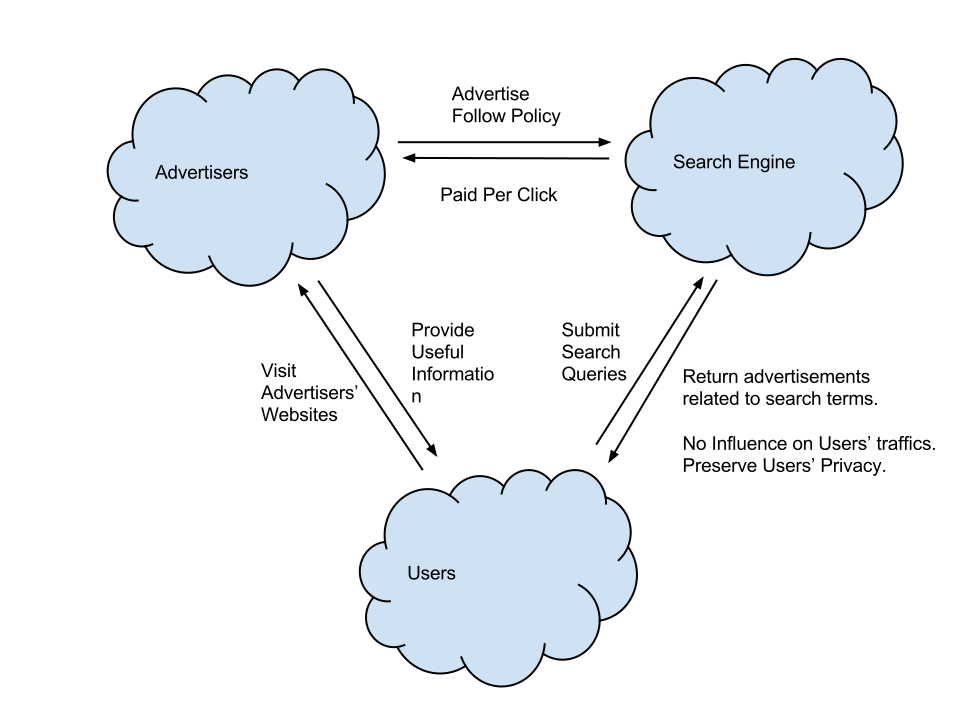
\includegraphics[width=.5\textwidth]{fig/three-parties}
	\label{fig:sem-model}
	\caption{Three-paries relationships in SEM}
\end{figure}

\subsection{Cloaking Detection}
Talk about cloaking detection related work here.
According to ~\cite{wang2011cloak}, they used the precision rate to measure the cloaking distribution on the search enginee hot terms. However, precision is highly depends on TRP and FPR. Using the precision to measure the distribution is fundamentally wrong method to do that. One of the right ways is using the TPR and FPR to measure the distribution. Another mistake they made is using constant numbers to measure time-based data without doing cross-validation. One way to do that is using the cross-validation or time-based adaptive parameter to solve this problem. 

Tree party relationships in SEM field. 
To better understanding the advantages of our crowdsourcing model, we briefly introduce the relationships in Search Enginee Markering (SEM). 

Traditional cloaking detection model only targets SEO field, our simhash based cloaking detection method could work both on SEO and SEM field. The main difference between the SEM and SEO is that every link in SEM is "pay per click". This indicates that  traiditional crawler will increase the advertisers payments by clicking the search result links and collecting data. If the cralwers first collect the landing page of the search result links then visit urls to collect data. The crawlers won't find the referal cloaking accoding to defination of referal cloaking. However, in our crowdsoucing model, the data we collected is from real users' clicks. Advertisers wouldn't pay extra money because of data collection. 
Model based on crowdsourcing could preserve the three party relationships between Users, Search Enginee Providers and Advertisers.



\subsection{Simhash}
Talk about simhash related work here. \\
Simhash~\cite{charikar2002similarity}  is a locality sensitive hash algorithm.
It is widely used by search engine to detect near duplicate of websites.


Show what simhash does and how they are used in the past.

Some embedded literal typeset code might 
look like the following :

{\tt \small
  \begin{verbatim}
  int wrap_fact(ClientData clientData,
  Tcl_Interp *interp,
  int argc, char *argv[) {
    int result;
    int arg0;
    if (argc != 2) {
      interp->result = ``wrong # args'';
      return TCL_ERROR;
    }
    arg0 = atoi(argv[1]);
    result = fact(arg0);
    sprintf(interp->result,``%d'',result);
    return TCL_OK;
  }
  \end{verbatim}
}

Now we're going to cite somebody.  Watch
for the cite tag.
Here it comes%~\cite{Chaum1981,Diffie1976}.
The tilde character (\~{})
in the source means a non-breaking space.
This way, your reference will
always be attached to the word that preceded it,
instead of going to the
next line.


\subsection{Simhash in Cloaking Detection}
Show the story here please!

1.what is the technical challege that we are addressing? compared to traditional
methods.

a. attacker could incrementally block inspector IP
b. crowdsourcing is cheap, compared to buying new IPs
c. crowdsourcing match user distribution and user habbit on web ~\cite{wang2011cloak}.

2. why we need simhash.
reduce volume of data, and collect enough information for cloaking detection.


3. what is user incentive?
build an extension to help user understand whether this website is
safe/compliant or tricking user by cloaking

user privacy is protected and can get better service.






\section{Simhash-based Website Model}
\label{s:swm}
\subsection{Distance Approximation}
Simhash~\cite{charikar2002similarity} is a hash function family that maps a high dimension dataset into fixed
bits and preserves the following attribute:

Suppose P and Q are probability distributions over L, 
\begin{multline}
  EMD(P, Q) \le E[d(h(P), h(Q))] \\
  \le O(\log{n}\log{\log{n}})EMD(P, Q).
\end{multline}

This equation is telling us that the hamming distance between simhash of set
\b{P} and set \b{Q} is an approximation of Earth Moving Distance(EMD) between set P
and Q. Charikar~\cite{charikar2002similarity} give the formal proof that the
hamming distance of sets represents the cosine similarity.
~\cite{manku2007detecting} implements an algorithm for creating text-based
simhash for a website.


\subsection{Computation}
In order to detect cloaking, we need to capture the bahavior and similarity that
a same website maintains. That is to say, we not only need to look at the text-based simhash,
but also dom-based simhash. We implemented the text-simhash algorithm described
in ~\cite{manku2007detecting}, which extract words, bi-gram, tri-gram set
(repeated elements only recorded once) from a website and compute simhash using
simhash algorithm described in ~\cite{charikar2002similarity}.

There is no current algorithm for generating dom simhash. Therefore, we design
an algorithm to perform this task. For each dom tree, we record the node set, as
well as the child parent pair set. The node set tells us information about what
tag is present in this page, and child parent pair tells us how these tags are
organized.

% you can also use the wonderful epsfig package...
\begin{figure}[t]
  \centering
  \begin{subfigure}
    \centering
    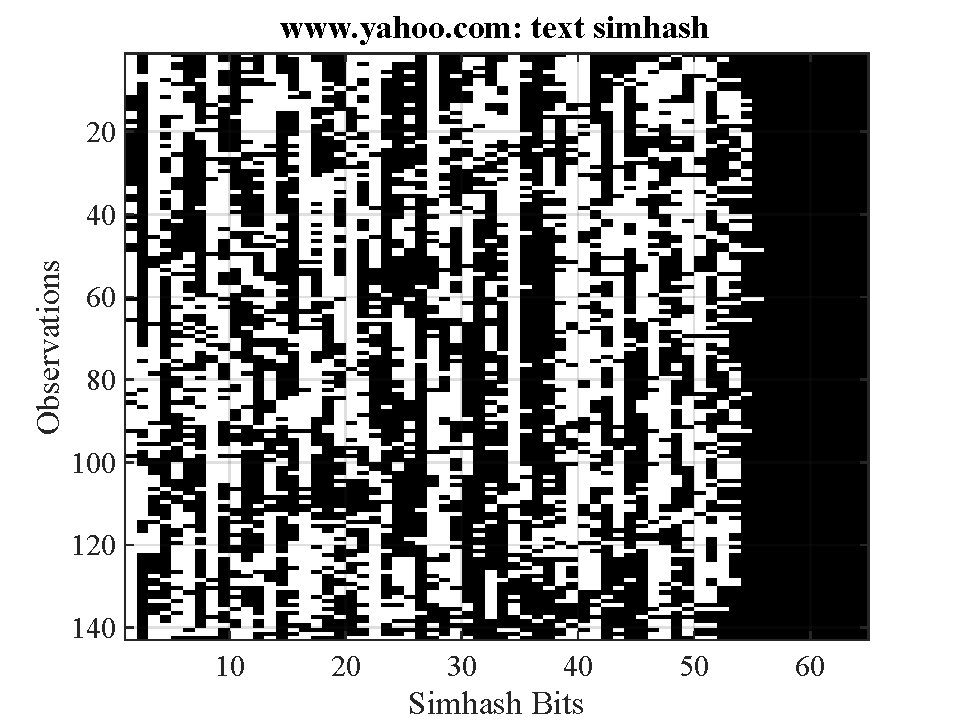
\includegraphics[width=.5\textwidth]{fig/yahoo-text-user}
    \label{fig:yahoo-text-user}
  \end{subfigure}%
  \begin{subfigure}
    \centering
    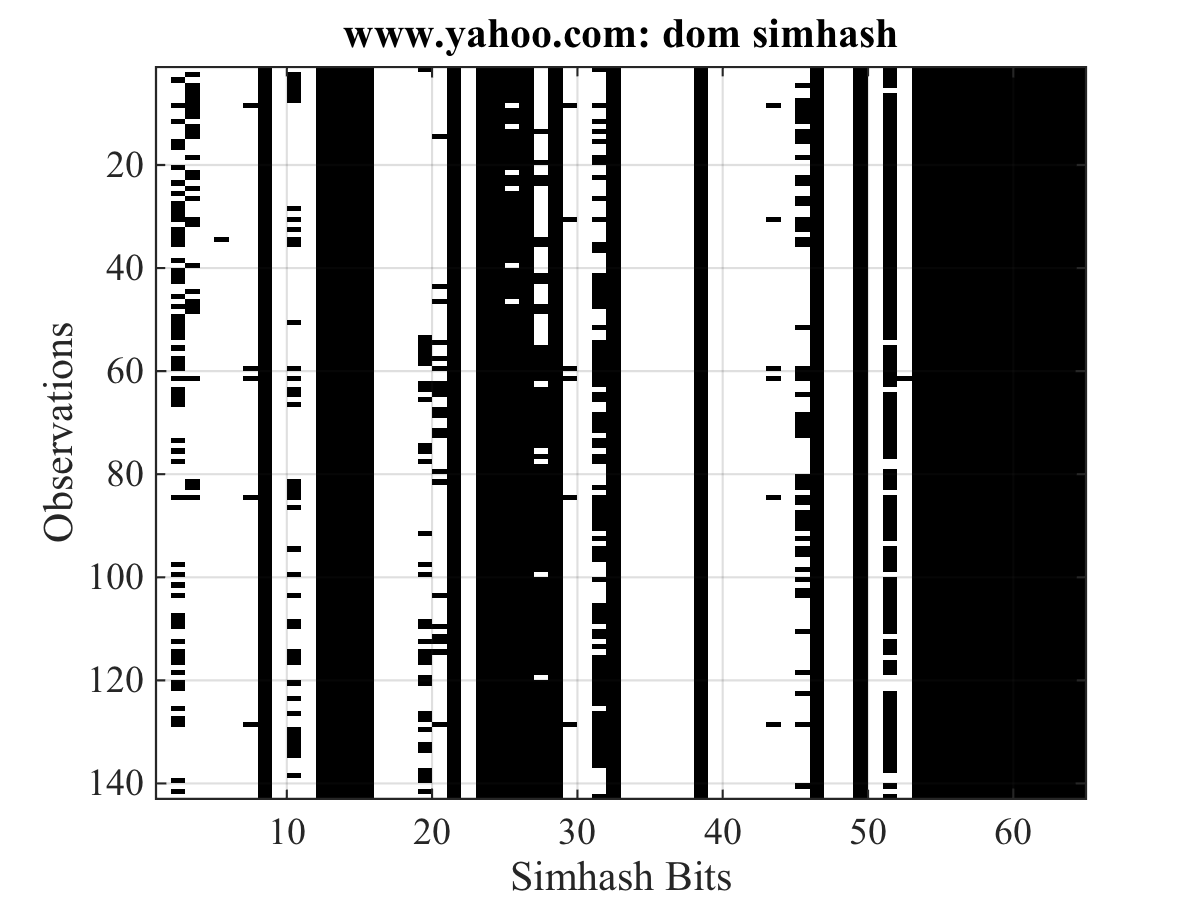
\includegraphics[width=.5\textwidth]{fig/yahoo-dom-user}
    \label{fig:yahoo-dom-user}
  \end{subfigure}
  \caption{Yahoo simhash changes over 7x24 period Feb.1 - 7, 2015}
  \label{fig:yahoo-simhash}
\end{figure}





It is pretty straightforward from ~\autoref{fig:yahoo-simhash} that,
text simhash changes rapidly, indicating dynamic nature of this
website, and dom simhash changes relatively slow and less.

Till now, we have demonstrated the algorithm we are using to generate
text-simhash and dom-simhash out of a website. Based on our observation, the
text-simhash may change rapidly, while dom-simhash relatively remain the same.


\subsection{Aggregating / Clustering}
Assume we are monitoring the same website over a period of time. This website
have dynamic changes all the time. But there can be another kind of change -
whole page change. In this case, it is reasonable to first separate them apart
and look at each of them.


Hamming distance is a special case of Euclidean distance. We can take the
average to represent the center of these points.


Using the hamming distance measure on a dimension of 64-bit.


For different websites, simhash can be considered as an algorithm to map them to
a 64-bit number randomly ~\cite{manku2007detecting}. For the same website,
simhash measures the similarity between them.



\begin{figure}[t]
  \centering
  \begin{subfigure}
    \centering
    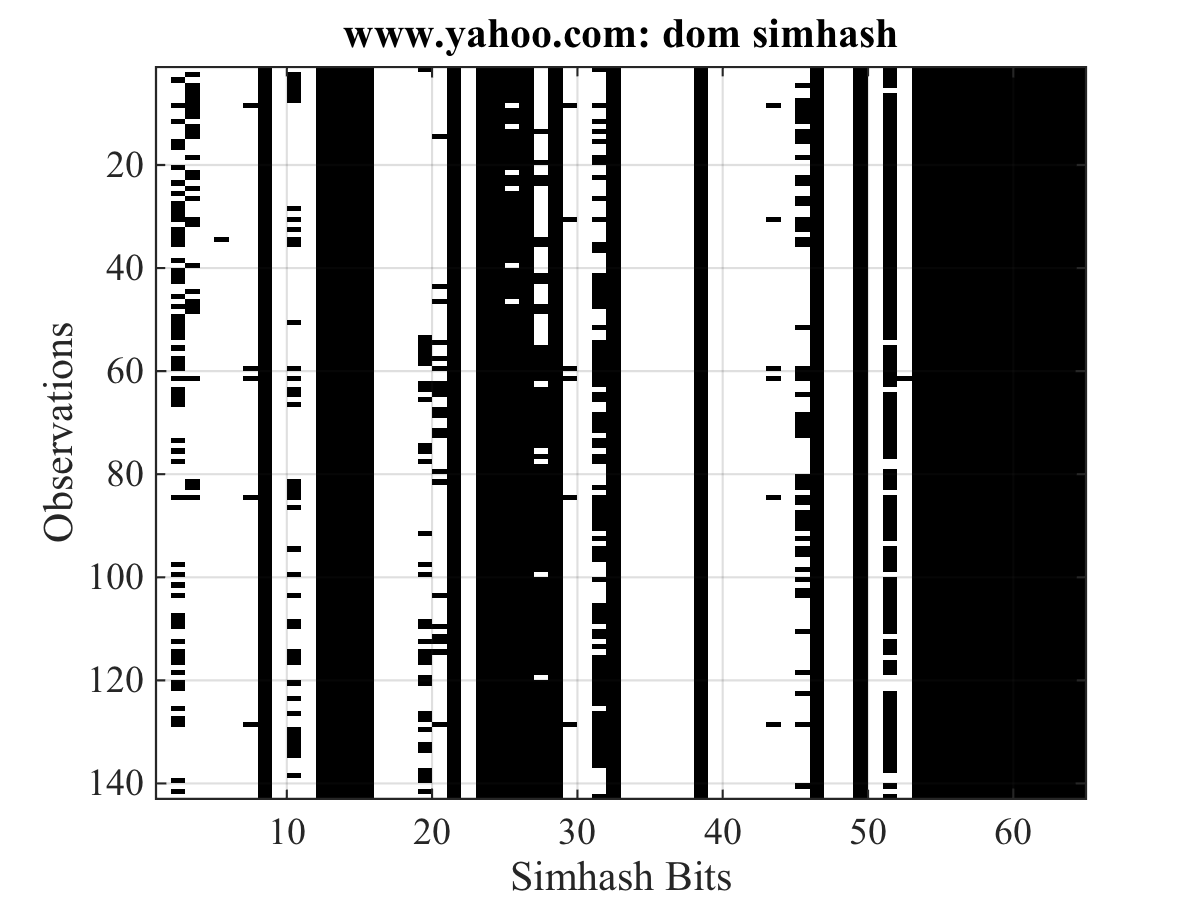
\includegraphics[width=.5\textwidth]{fig/yahoo-dom-user}
    \label{fig:yahoo-dom-user}
  \end{subfigure}%
  \begin{subfigure}
    \centering
    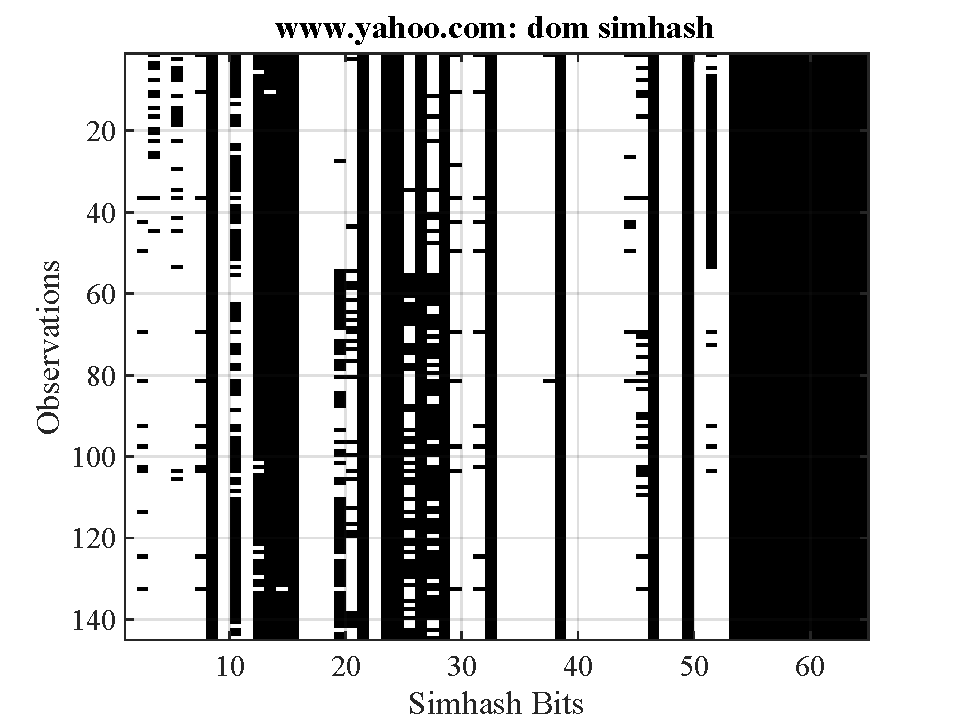
\includegraphics[width=.5\textwidth]{fig/yahoo-dom-google}
    \label{fig:yahoo-dom-google}
  \end{subfigure}
  \caption{Comparison of user and google seen dom simhash}
  \label{fig:yahoo-simhash}
\end{figure}




Different from ~\cite{manku2007detecting}, we not only want to know whether two pages are
duplicate, we also want to know the patterns of these simhash. In this work, we employ
hierarchical clustering to do this job.

In hierarchical clustering uses a set of dissimilarities for the n objects being clustered.
Initially, each object is assigned to its own cluster and then the algorithm
proceeds iteratively, the complete linkage method finds similar clusters.

In order to decide the number of clusters to take in hierarchical clustering
(when to stop), we use inconsistent coefficient.


L1 norm : sum of the differences in
each dimension

considerations of significance, we ask whether this is an unusual result or
whether it could have arisen merely by chance


The inconsistency coefficient characterizes each link in a cluster tree by
comparing its height with the average height of other links at the same level of
the hierarchy. The higher the value of this coefficient, the less similar the
objects connected by the link.

One way to determine the natural cluster divisions in a data set is to compare
the height of each link in a cluster tree with the heights of neighboring links
below it in the tree.

linkage metric: hammming
method: Unweighted average distance (UPGMA)
cutoff: inconsistent value less than c
pick inconsistent value now!!!!!

learning 1.1
detection 2.0


\begin{gather*} \label{npa}
  d(u,v) = \min(dist(u[i],v[j])) \\
  \text{for all points i in cluster u and j in
  cluster v. }
\end{gather*}
This~\autoref{npa} is known as the Nearest Point Algorithm.

Single-linkage clustering is one of several methods of agglomerative
hierarchical clustering. In the beginning of the process, each element is in a
cluster of its own. The clusters are then sequentially combined into larger
clusters, until all elements end up being in the same cluster. The stop
criterion is the distance one.




It can get tricky typesetting Tcl and C code in LaTeX because they share
a lot of mystical feelings about certain magic characters.  You
will have to do a lot of escaping to typeset curly braces and percent
signs, for example, like this:
``The {\tt \%module} directive
sets the name of the initialization function.  This is optional, but is
recommended if building a Tcl 7.5 module.
Everything inside the {\tt \%\{, \%\}}
block is copied directly into the output. allowing the inclusion of
header files and additional C code." \\

Sometimes you want to really call attention to a piece of text.  You
can center it in the column like this:
\begin{center}
  {\tt \_1008e614\_Vector\_p}
\end{center}
and people will really notice it.\\

\noindent
The noindent at the start of this paragraph makes it clear that it's
a continuation of the preceding text, not a new para in its own right.


Now this is an ingenious way to get a forced space.
{\tt Real~$*$} and {\tt double~$*$} are equivalent. 

Now here is another way to call attention to a line of code, but instead
of centering it, we noindent and bold it.\\

\noindent
{\bf \tt size\_t : fread ptr size nobj stream } \\

And here we have made an indented para like a definition tag (dt)
in HTML.  You don't need a surrounding list macro pair.
\begin{itemize}
  \item[]  {\tt fread} reads from {\tt stream} into the array {\tt ptr} at
    most {\tt nobj} objects of size {\tt size}.   {\tt fread} returns
    the number of objects read. 
\end{itemize}
This concludes the definitions tag.

\subsection{Model Selection}


\begin{table*}[!th]                                                     
  \centering                                                            
  \scriptsize                                                           
  \begin{tabular}{lllllllllll}
  \toprule
  & \multicolumn{2}{c}{\textbf{Normal}}
  & \multicolumn{2}{c}{\textbf{Lognormal}}
  & \multicolumn{2}{c}{\textbf{Exponential}}
  & \multicolumn{2}{c}{\textbf{Gamma}}
  & \multicolumn{2}{c}{\textbf{Logistic}}\\

  \textbf{Website(Hash Type)\textbackslash Model}
  & AD-value
  & P-value
  & AD-value
  & P-value
  & AD-value
  & P-value
  & AD-value
  & P-value
  & AD-value
  & P-value \\
  \midrule
  digg.com T & 0.617 &  0.100 & 0.481 &  0.219 &
  14.851 & < 0.003 & 0.538 &  0.186 & 0.531 &  0.131\\ 
  digg.com T & 0.227 &  0.806 & 0.179 &  0.914 &
  19.690 &  < 0.003 & 0.198 &  > 0.250 & 0.250 & >0.250\\
  yahoo.com T & 0.192 &  0.893 & 0.263 &  0.692 &
  35.828 & <0.003 &   0.231 & >0.250 & 0.222 & >0.250\\
  amazon.com T & 0.720 &  0.058 & 0.323 &  0.520 & 
  27.754 & <0.003 &  0.436 & >0.250 & 0.642 &  0.058\\
  reddit.com T & 0.373 &  0.411 & 0.331  & 0.509 & 
  35.063 & <0.003 & 0.340 & >0.250 & 0.361 & >0.250\\
  yacombinator.com T & 0.473 &  0.237 & 0.516 &  0.186 &
  37.551 & <0.003 & 0.519 &  0.204 & 0.583 &  0.089\\

  digg.com D & 0.319 &  0.372 & 0.348 &  0.305 &
  1.491 &  0.021 &  0.402 & >0.250 & 0.363 & >0.250\\
  yahoo.com D & 0.531 &  0.168 & 0.392 &  0.366 &
  18.837 & <0.003 & 0.441 & >0.250 & 0.584  & 0.088\\
  amazon.com D & 1.519 & <0.005 & 0.916 &  0.019 &
  22.083 & <0.003 & 1.052 &  0.009 & 0.548 &  0.114\\
  amazon.com D & 0.483 & 0.117 &  0.504 & 0.104 &
  1.741 & 0.010 & 0.601 & 0.128 & 0.523 & 0.115\\

\end{tabular}

                                     
  \caption{Model statistics for selected websites}
  \label{tbl:para-select}                                         
\end{table*}                                                            


This table ~\autoref{tbl:para-select} shows the Anderson-Darling (AD) value and P-value for each model.
A common rule used in model selection is pick the model which has the smallest
value with P-value greater than 5\%. Each row in the table represents one
website. From the statistics of these websites, we choose normal distribution
for text simhash and Lognomal distribution for dom simhash.

In the simhash based cloaking detection model, input from the user is simply simhash. How to compare against the simhashs that is already collected?

One simple way is to compute the average distance from this simhash to all the observed simhashs. The next step is then to tell whether this distance is reasonable. 

The text distribution follows lognormal distribution.
After mannual check of those results.




You have to run {\tt latex} once to prepare your references for
munging.  Then run {\tt bibtex} to build your bibliography metadata.
Then run {\tt latex} twice to ensure all references have been resolved.
If your source file is called {\tt usenixTemplate.tex} and your {\tt
bibtex} file is called {\tt usenixTemplate.bib}, here's what you do:
{\tt \small
  \begin{verbatim}
  latex usenixTemplate
  bibtex usenixTemplate
  latex usenixTemplate
  latex usenixTemplate
  \end{verbatim}
}




\section{Framework}
\label{s:framework}


1. adaptive parameter. websites change dynamically. It's hard to give a contant  parameter for the dynamic changes on the website.
2. compare with other work. Result rate could be better. But dataset is different. Previous method probably will get lower deteciton rate on current data. 


\section{Experiment}
\label{s:experiment}



\subsection{Dataset}

\XXX{plot simhash of known cloaking}

Because we want to measure cloaking in SEO and SEM, we have compiled a list of
cloaking words, from the policies specified by Adwords, inspired by the words
collection process in ~\cite{wang2011cloak}. We have looked at the policies, and
collected \XXX{N} words, from ad network abuse, adult abuse, alcohol abusive, dangerous behavior
abuse, dishonest behavior abuse, health abuse, gambling abuse.

Step 1: For each word, with chrome user agent, we click and visit search results and advertisements on first
twenty pages. \\
Step 2: For the landing pages collected in step 1, with google bot user agent, we visit them 6 times at an
interval of around 20 miniutes.

6 copy is collected because we need to model the distribution of websites. It is
a tradeoff between space and precision. If we want to model the website better,
we may want to collect as many examples as possible.


We randomly sample 600 websites from the dataset, for 10 times. This results in
5726 websites. We manually label them and \XXX{cloaking}, \XXX{not}, percentage
for each is.


\subsection{Groundtruth}

We remove the failure websites and this results in 
113242 urls, exact match, parameter different are counted.
98390 sites, parameters ignored. Later we will use the latter parameter because
it makes more sense.


Visit \XXX{1000} search words, for collected search urls, we have collected
\XXX{130K} URLs.


\XXX{Filter?}
Maybe not
\bf{Step 1: Filter}

In order to get groundtruth, we follow a similar process employed in
~\cite{lin2009detection}, we first filter the results and get rid of the highly reputated ones. We write a
script to query the WOT API, and remove websites with combined score 80
(which is a pretty high score) and the results are \XXX{N} urls after that.

for advertisements, after filtering, there are 2279 (score 60) urls
remained.\XXX{Problematic because I haven't merged them}

for search results, after filtering, there are 90120 (60) urls remained.
\XXX{Problematic because I haven't merged them}


\bf{Step 2: De-duplication}

71116 urls

62042 websites


This results in \XXX{Some} links. Then we compare the text simhash and dom
simhash, remove those which are exactly duplicate of one of the simhash observed
by Google. After this step, we have \XXX{N} url left.

For advertisements, after deduplication, there are 997 (score 60) urls remained.

For search results, after deduplication 37155 urls, 35444 websites remained.


\bf{Step 3: Random Sample and Labeling}


Then we randomly select 1000 urls from the dataset, and label them, after
labeling, we found \XXX{N} cloaking sites and \XXX{M} dynamic websites.
These are the groundtruth we used to label our data.

\subsection{Detection and Evaluation}
We have detected.

We manually examine the results and found \XXX{N} are actually cloaking.

For SEO and SEM, the cloaking rate is 5\% and 3\% in the dataset collected by
us.




We see a lower clokaing rate compared to XXX, may be because Google has done
something to this. However, this problem still remains.


For the United States, web search dataset.

The advertisements are
before dedup: 4381
after dedup: 1487



\section{Discussion}
\label{s:discussion}

In this part, we will discuss two kinds of deployment of simhash based cloaking detection system: server-based and crowdsoucing.

\subsection{Server-based cloaking detetion system}
In server-based cloaking detection system,
we first collect targeted search terms includes commecial terms, cloaking oriented terms and hot trend words.
Using these search terms, the cralwer extracts the search results from the search engines for seven times.
In six times, the crawler disguises as Google crawler by using the Google Agent and crawl data. With this data that
is crawled from Google view, the system uses the simhash method to model the websites. The last
time, the crawler disguises as normal user by using user agent. The system compares simhash value from user view and
website model learned from Google view. From the comparsion result, the system judges if the website is cloaking
or not. 
Server based cloaking detection system has pros and cons. The deployment of server based cloaking dectetion system
is pratical and could be deployed
easily. The tradeoff of easy deployment is inefficient in IP cloaking detection. Usually, the servers IP addresses
are in a range,  scammers could find this range and serve benign content to crawlers. One solution is buying numerous IP addresses
from ISP providers and distributing IP addresses as users distribution. This increases cloaking detection cost. In
addition, distributing IP addresses as users distribution is hard. Further, server-based cloaking detection system is infeasiable
to detect cloaking in search engine marketing(SEM). As we mentioned, using the crawlers to visit websites in SEM field
increases the advertisement cost of websites. Moreover, different websites has different changing periods. For example, Yahoo website
updates very quickly. Apple website updates slowly. Finding different crawling periods for different websites is difficult. 

\subsection{Crowdsourcing}
Crowdsourcing cloaking detection system includes user-side and server-side component. In user side, users needs to install the cloaking
detection extension in their browers. While users click search results and view websites, the extention calculate the simhash value based on 
website content and layouts. After calculation, extension packs URL and simhash value and sends to server. Server passively receives (URL, simhash value)
pairs from users. Server also utilizes crawlers to extract content several times in this URL from search engine view (crawler uses Google bot agents).
Server uses these extract content to model the website. From the comparison result between (URL, simhash value) from users and website model,
server could decide if the website is cloaking or not. From previous study, cloaking includes phishing and malware downloading. Based on cloaking
detection result, server categorizes cloaking and update blacklists in browsers' extensions. Updating blacklists and warning users phishing and
malware downloading is users incentive to install our extension.

Previously, we describe our crowdsoucing workflow. Next, We discuss the pros and cons for this approach. The first advantage is privacy. Instead of solicting
website content from users, the system solicited a 64 bits simhash value from users. From this 64 bits value, system couldn't do reverse engineering to
get original content. In addition, the system could intergrate with RAPPOR~\cite{erlingsson2014rappor}, which protect the privacy of URL.
Because the workflow is similar to safe browsing API ~\cite{rajab2013camp} , we argue that this can be easily
extended in current framework, the only different is that (URL, simhash value)
pair is processed through RAPPOR to achieve anonymity.

In addition, the crowdsouring deployment introduces low traffic. Browsers only send a 64 bits value for
each URL. This won't jam traffic. Further, the crowdsoucing deployment wouldn't affect the model of SEM. Each click on advertisements of search engines is
from real users instead of crawlers. Advertisers don't need to pay extra money for cloaking detection. 


Employ RAPPOR~\cite{erlingsson2014rappor} to provide user privacy gurantee.

pros: 	1.privacy 2.Low traffic. 3.SEM 4.Distributed computation 
5. Remove the need to do redirect cloaking detection, leveraging the feature
that the end goal of attackers is to reach user
6. could decide crawl period passively based on user clicks, data received are
based on real user’s clicks, say, website traffic
%
%cons: user incentives. 
%Solution: Plugin to detect suspicious websites. API


\begin{figure}[t]
  \centering
  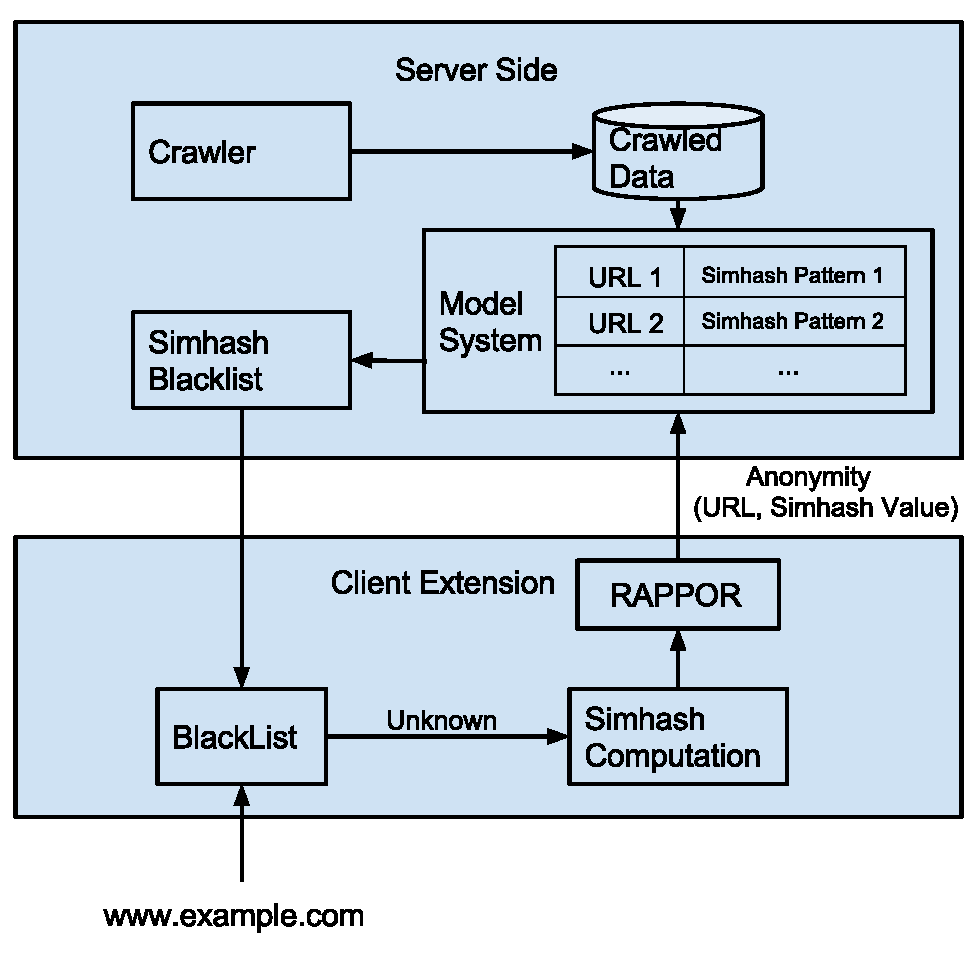
\includegraphics[width=.45\textwidth]{fig/crowdsourcing-cloaking-detection-system}
  \caption{Workflow of crowdsource cloaking detection sysetem}
  \label{fig:workflow}
\end{figure}


The workflow ~\autoref{fig:workflow} is to collect page contents simhash on the user side, and compare
them to simhash of the same link from ad serving company to find cloaking. When
the differences of the simhashes are significantly large, the page is marked
cloaking. We generate two simhash for page content and structure respectively.
Intuition behind this is, simhash difference between different sites are larger
than different visits of the same site. We build a two-phase system to detect
cloaking: cluster learning phase, and cloaking detection phase. In the cluster
learning phase, an ad company visit urls and generate simhash from its content
with its owned IP, and learn pattern and distribution of the simhashes, i.e.
simhash-based website model. In the cloaking detection phase, the ad company
collects simhash from its users. Compare them with learned patterns, return
cloaking score or mismatch



\section{Acknowledgments}

A polite author always includes acknowledgments.  Thank everyone,
especially those who funded the work. 

\section{Availability}

It's great when this section says that MyWonderfulApp is free software, 
available via anonymous FTP from

\begin{center}
{\tt ftp.site.dom/pub/myname/Wonderful}\\
\end{center}

Also, it's even greater when you can write that information is also 
available on the Wonderful homepage at 

\begin{center}
{\tt http://www.site.dom/\~{}myname/SWIG}
\end{center}

Now we get serious and fill in those references.  Remember you will
have to run latex twice on the document in order to resolve those
cite tags you met earlier.  This is where they get resolved.
We've preserved some real ones in addition to the template-speak.
After the bibliography you are DONE.

{\footnotesize \bibliographystyle{acm}
%\bibliography{../common/bibliography}}
\bibliography{ruian,weiren}}

\theendnotes

\end{document}







